\documentclass[10pt,twocolumn]{article}
\usepackage[letterpaper,margin=0.72in,columnsep=0.24in]{geometry}
\usepackage[T1]{fontenc}
\usepackage[utf8]{inputenc}
\usepackage{times}
\usepackage{microtype}
\usepackage{booktabs}
\usepackage{graphicx}
\usepackage{stfloats}
\usepackage{float}
\usepackage[font=small,labelfont=bf,skip=3pt]{caption}
\usepackage[round]{natbib}
\setlength{\bibsep}{0pt}
\usepackage[most]{tcolorbox}
\usepackage[hidelinks]{hyperref}
\usepackage{titlesec}
\titlespacing*{\section}{0pt}{4pt}{1pt}
\titleformat{\section}{\normalsize\bfseries}{\thesection}{0.5em}{}
\setlength{\parskip}{2pt}
\setlength{\parindent}{0pt}
\setlength{\textfloatsep}{6pt}
\setlength{\dbltextfloatsep}{6pt}
\newtcolorbox{hypbox}{colback=gray!8,colframe=gray!60,boxrule=0.4pt,arc=1pt,left=3pt,right=3pt,top=2pt,bottom=2pt}

\title{\vspace{-0.62in}\large\textbf{Can LLM Agent MPs Reproduce a Language Convention\\That Split the Polish Parliament?}\\[2pt]\normalsize A Real-World Test for Agent Simulations of Social Conventions}
\author{\normalsize Antoni Czolgowski \quad CSCI 7000 NLP for Cultural Analytics, Proposal 2, 19 October 2026}
\date{\vspace{-0.32in}}

\begin{document}
\maketitle

\section{Motivation and research questions}
In Polish you live \emph{w Polsce} (``in Poland'') and \emph{w Niemczech} (``in Germany''), but for centuries you lived \emph{na Ukrainie}, literally ``on Ukraine'', with the preposition Polish uses for regions and also for a few countries (\emph{na Litwie}, \emph{na Węgrzech}). Both forms mean the same place, so the choice between them is a pure \emph{convention}: a way of saying something that people keep mainly because others keep it. When Russia started full invasion on 24 February 2022, this convention suddenly carried a message. For many speakers, \emph{w Ukrainie} came to express respect for Ukraine as a sovereign state, and in July 2022 the Polish Language Council encouraged its wide use \citep{rjp2022}. A change like this, with a known start and a full record of who changed and who did not, is a rare chance to test whether LLM agents that stand in for people make the choices those people made.

In the Sejm, the lower house of the Polish parliament, the choice turned political. In March 2022 an MP of PiS, the governing right-wing party, said that ``\emph{w Ukrainie} to rusycyzm'' (``\emph{w Ukrainie} is a Russianism''). In October 2022 an MP of KO, the main liberal opposition, told a committee: ``ja też mówię \emph{na Ukrainie}, tylko że w Sejmie wszyscy mówią \emph{w Ukrainie}, więc chciałabym, żebyśmy się dostosowali'' (``I also say \emph{na}, but in the Sejm everyone says \emph{w}, so I would like us to adapt''). The second quote is the textbook mechanism of convention change, said out loud: people adopt a form because they see others use it. In experiments with arbitrary names, a committed minority of about 25\% is enough to tip a whole group \citep{centola2018}. The Sejm lets me ask whether that happens with a real convention that carries political identity.

\textbf{Why simulate MPs at all?} LLM agents are now used as stand-ins for people: as survey respondents \citep{argyle2023}, as simulated individuals \citep{park2024}, to predict the results of social science experiments \citep{ashokkumar2026}, and as whole populations in which researchers watch conventions form and tip \citep{ashery2025,flint2026}. These studies make claims about how conventions and norms spread among humans, so they are only as good as the agents' resemblance to the people they stand for. For convention change that resemblance has three parts: \emph{who} adopts a new form, \emph{when}, and \emph{how much} each person follows the one before. Critics warn that simulations exaggerate effects \citep{ashokkumar2026,feroz2026} and may only replay what the model saw in training \citep{barrie2025}, but most checks compare agents with survey averages or lab games, not with real decisions in context. I propose a direct check: place the agent at the exact moment a real person made a choice, give it the context that person had, and compare its choice with theirs. The Sejm transcripts make this check possible for all three parts: they show which form each MP used (\emph{who}), on which day (\emph{when}), and what the speakers right before them had just said (\emph{how much} they follow others). The question also matters on its own: LLMs increasingly draft political text, and a model that defaults to one form quietly takes a side in a live dispute.

\begin{hypbox}
\textbf{RQ1 (people).} After the invasion, did \emph{w Ukrainie} tip in the Sejm or split along party lines, and do MPs follow the form the previous speaker used?\\[2pt]
\textbf{RQ2 (agents).} When open LLMs are placed at the real choice points, with the real debate before them and the MP's identity, do they choose the form the MP chose?\\[2pt]
\textbf{H1 (flattened politics).} Agents rank the parties in the same order as real MPs, from the party that uses \emph{w} most (Lewica, the left) to the one that uses it least (Konfederacja, the right), but the differences between parties are much smaller than in reality. \emph{Disconfirmed if} the agents reproduce the real differences: regressing each party's log-odds of \emph{w} for the agents on the same quantity for real MPs gives a slope whose 95\% CI includes 1 (1 = the same differences as real MPs, 0 = no differences at all).\\[2pt]
\textbf{H2 (over-alignment).} Agents copy the form used in the speeches just before them more than real MPs do. \emph{Disconfirmed if} the odds ratio (OR) for \emph{w} after swapping \emph{w} and \emph{na} in those speeches has a 95\% CI that overlaps the CI of the real MPs' previous-speaker OR.\\[2pt]
\textbf{H3 (no individual signal).} Knowing who the MP is does not let agents predict the choice better than knowing the MP's party. \emph{Disconfirmed if} the agent's AUC (the probability that a real \emph{w} speech gets a higher P(\emph{w}) than a real \emph{na} speech; 0.5 = chance) has a 95\% CI above that of a lookup of the party's real rate.
\end{hypbox}

\section{Data}
\textbf{Polish Parliamentary Corpus} \citep[PPC;][]{ogrodniczuk2018}: the official written transcripts of Sejm plenary sittings and committee meetings. These are records of spoken debate edited by stenographers, in TEI XML with the speaker, role and party club of every turn. I used the 9th and 10th terms (2.9\,GB zipped, 5,940 Sejm documents, uses from Nov 2019 to Apr 2025), with MP biographies from the official Sejm API. \emph{Permissions:} official documents are not protected by Polish copyright law and the annotations are CC BY; these are public statements of public officials, so there is no IRB question, and the models generate no text.

\section{Language features (operationalization)}
The unit of analysis is one locative phrase: \emph{w} or \emph{na} followed by \emph{Ukrainie}, found with a regular expression. After these prepositions the form \emph{Ukrainie} always refers to Ukraine as a place, so the only noise is MPs quoting the phrase as a word (``\emph{w Ukrainie} to rusycyzm''); I flag these by the quotation marks and drop them. The choice is a good measure of the convention because the two forms are a minimal pair (same meaning, position and length): only the convention, and what the speaker signals by it, differs. Three features turn the counts into a test. (1) \textbf{Controls:} the same choice before Lithuania, Belarus, Slovakia, Hungary and Latvia, which also take \emph{na}; if MPs switch there too, the change is about the language, not about Ukraine. (2) \textbf{The previous form:} for each use, the form the last other speaker in the same sitting used, which measures alignment. (3) \textbf{The agents' choice:} P(\emph{w}) is the model's probability of the continuation `` w Ukrainie'' divided by the sum for `` w Ukrainie'' and `` na Ukrainie'', written as in the transcript. I score the whole phrase because the next word \emph{w} alone also covers \emph{w Polsce}.

\begin{equation*}
P(w) = \frac{P(c_w \mid x)}{P(c_w \mid x) + P(c_{\mathit{na}} \mid x)}
\end{equation*}
\begin{equation*}
P(c \mid x) = \prod_{t=1}^{|c|} P(c_t \mid x, c_{<t})
\end{equation*}
where $x$ is the prompt including the pre-filled reply, $c_w$ and $c_{\mathit{na}}$ are the tokens of `` w Ukrainie'' and `` na Ukrainie'' (three tokens in every model), and each factor $P(c_t \mid x, c_{<t})$ is the model's probability of the next token given everything before it. The next-word version keeps only the first factor ($t=1$).

\section{Feasibility test}
\textbf{People (RQ1): the convention split instead of tipping.} The PPC has 6,431 \emph{w/na} uses before the six country names, 4,068 of them before \emph{Ukrainie}. Before the invasion only 3 of 211 (1.4\%) were \emph{w}. After it, 31\% of 3,857 were, and the share then stopped growing: 30.2\% under the PiS government and 32.6\% after the KO-led coalition took over in November 2023. The control countries barely moved (Belarus 8\%, Slovakia 11\%, the other three 1--2\%), so the change is about Ukraine and not about the preposition. A minority of about 30\% kept using \emph{w} for three years without tipping the room, more than the 25\% that tipped groups in the experiments. Figure~1a shows why: the convention became a party marker. Under the KO-led government, \emph{w} was 79\% in Lewica (the left), 56\% in KO, 47\% in Polska 2050, 22\% in PSL, 11\% in PiS and 2\% in Konfederacja (the right), and PiS and Konfederacja moved \emph{away} from \emph{w} over time. Within the split, individuals mix (163 of the 230 MPs with five or more uses used both forms) and respond to the room. In a logistic regression with party, government period, committee vs plenary and months since the invasion, with standard errors clustered by speaker, an MP is more likely to say \emph{w} right after another speaker did (OR 1.63, 95\% CI [1.26, 2.10], $n$=2,456). This is a modest alignment effect, the tendency of speakers to reuse each other's words \citep{pickering2004}.

\begin{figure*}[t]\centering
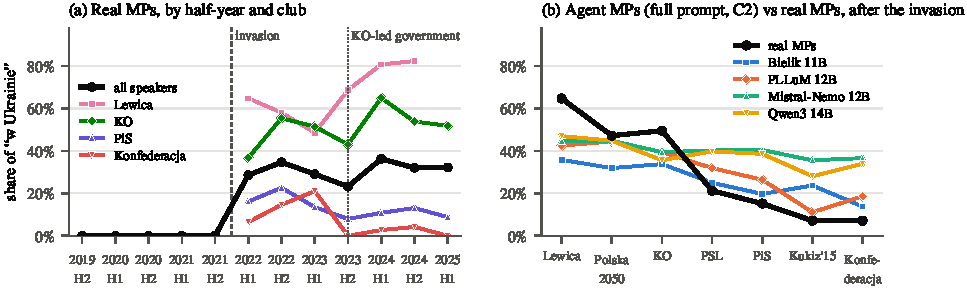
\includegraphics[width=\textwidth]{fig1.pdf}
\caption{(a) Share of \emph{w Ukrainie} in the Sejm by half-year, for all speakers and four party clubs (club lines start after the invasion and show half-years with at least 15 uses). (b) Mean P(\emph{w}) of each agent with the full prompt (C2), against the real share by club after the invasion. Clubs are ordered by the real share.}
\end{figure*}

\begin{table}[t]\centering\small\setlength{\tabcolsep}{2.4pt}
\begin{tabular}{@{}lcccc@{}}\toprule
 & Bielik & PLLuM & Mistral & Qwen3 \\ \midrule
AUC, C0 / C1 & .64/.69 & .61/.65 & .59/.60 & .56/.56 \\
AUC, C2 full prompt & \textbf{.70} & .64 & .58 & .56 \\
\quad 95\% CI & [.65,.74] & [.60,.69] & [.55,.63] & [.51,.61] \\
\quad next word only & .60 & .58 & .55 & .49 \\ \midrule
Club order $\rho$ / slope (H1) & .96/.31 & .86/.49 & .71/.10 & .75/.17 \\
\quad slope 95\% CI & [.23,.48] & [.35,.67] & [.03,.17] & [.07,.34] \\
Club swap, \% of real gap & 18\% & 13\% & 2\% & 3\% \\
Flip OR (H2) & 4.3 & 8.2 & 20.0 & 7.5 \\
\quad 95\% CI & [2.2,7.1] & [5.1,14] & [8.1,48] & [3.6,14] \\
P(\emph{w}), pre-invasion & .11 & .16 & .26 & .41 \\
\quad same, date +3 years & .14 & .19 & .28 & .40 \\ \bottomrule
\end{tabular}
\caption{Agents vs MPs (800 choice points after the invasion, 87 before). On the same 800 cases, a lookup of the club's real rate (leave-one-out) has AUC .74 [.68, .78], and the MP's own earlier uses .82 [.77, .86] ($n$=625). Real MPs: slope 1, OR 1.63, pre-invasion P(\emph{w}) .014. 95\% CIs from 1,000 bootstrap resamples of speakers.}
\end{table}

\textbf{Agents (RQ2): in the MP's place.} I sampled the first use in each speech: 800 after the invasion (at most 80 per club and government period) and all 87 before it. Each model reads a prompt in four layers. The \emph{scene} gives the date, the sitting and the agenda item. The \emph{identity} gives the club, role and Sejm API biography, plus two excerpts of the MP's own earlier speeches that contain no country names; it never gives the MP's name. The \emph{room} gives the last three real speeches before the MP's turn. The \emph{task} asks the agent to speak. Appendix~A shows the template. The model's reply is then pre-filled with the MP's real words (150 words) up to the choice point, so the agent stands exactly where the MP stood, and nothing is generated. Conditions change one thing at a time: C0 scene only, C1 adds the club, C2 is the full prompt, C3 is C2 with \emph{w} and \emph{na} flipped in the earlier speeches, C4 is C2 with the club swapped to the other camp (e.g.\ PiS$\leftrightarrow$KO), and D1 is C2 with the date moved three years later, for the pre-invasion speeches. Four open models ran in bf16: Bielik 11B v2.3 \citep{ociepa2025} and PLLuM 12B \citep{kocon2025}, both built for Polish, Mistral-Nemo 12B \citep{mistral2024} and Qwen3 14B \citep{qwen2025}; 16,796 prompts took 56 minutes on one 48\,GB GPU slice of CU's Alpine cluster.

\textbf{H1 is supported: agents know the order, not the distance.} The best agent, Bielik, ranks the seven clubs almost exactly as the MPs do (Spearman $\rho$ = .96), but its average P(\emph{w}) runs only from 0.14 to 0.36, against the real 0.07 to 0.65 (Figure~1b). On the log-odds scale its slope is 0.31 (95\% CI [0.23, 0.48]), far below 1, so it keeps about a third of the real political distance; every model's CI excludes 1. The two non-Polish models barely separate the clubs at all. The swap test agrees: telling Bielik that an MP belongs to the other camp moves it by 18\% of the real gap between the two clubs, and Mistral and Qwen by 2--3\%.

\textbf{H2 is supported: agents follow the room far more than MPs do.} Flipping \emph{w} and \emph{na} in the earlier speeches multiplies the odds of \emph{w} by 4 to 20, depending on the model, while real MPs show 1.63, and no agent CI overlaps the human one ([1.26, 2.10]). This is the exaggeration found by \citet{ashokkumar2026}, now on real debate. The sample is small (42 cases have the form in the last three speeches), and the two numbers are not the same estimand (an experiment for agents, an observational association for people).

\textbf{H3 is supported: the agents miss the individual.} Grounding helps, as Bielik's AUC rises from .64 with the scene only to .70 with the full prompt. But no agent beats a simple lookup of the club's rate (.74), and the MP's own earlier choices reach .82. The information that identifies an individual MP exists in the record, and the agents do not recover it from a biography and two speech excerpts. This holds even when the name is there: because the room is the real transcript, the chair often announces the next speaker by name (336 of the 800 post-invasion prompts), and agents do no better on those cases (Bielik AUC .69 vs .70). They also have little sense of \emph{when}. Moving a pre-invasion speech three years later barely changes P(\emph{w}), and Qwen gives \emph{w} a 41\% chance before the invasion, when MPs used it 1.4\% of the time, an anachronism in the sense of \citet{underwood2026}. Scoring only the next word lowers every AUC (Table~1).

\textbf{Memorization check: no sign that the models know the transcripts.} If the models had seen the Sejm transcripts in training, they could simply recall what each MP said rather than simulate it \citep{chang2023}. I tested this with Min-K\% \citep{shi2024}, which averages a model's 20\% lowest token log-probabilities on a text; memorized texts have fewer surprising tokens, so they score higher. Transcript excerpts from 2022--23 could be in the training data, while most excerpts from 2025 come after the models' training cutoffs. For all four models the two groups score the same (120 excerpts each, all 95\% CIs of the difference include 0).

\section{Relation to existing work}
Most evidence on how conventions tip comes from games with arbitrary names, played by people \citep{centola2018} or by LLM populations \citep{ashery2025}. The LLM version is open to the critique that models recognize the game from training data \citep{barrie2025}, and new work shows that conventions can be tipped indirectly, through stepping-stone forms \citep{flint2026}. Language change has been traced in the French Revolution debates \citep{barron2018}, abolitionist newspapers \citep{soni2021} and online communities \citep{danescu2013}, without asking whether a model could reproduce it. Work on the validity of LLM simulations compares closed survey answers or experimental effects \citep{argyle2023,park2024,ashokkumar2026,feroz2026}. \textbf{What I add:} a test that scores agents at the exact moments of real choices against human baselines on the same scale, and a first testbed for it: a real convention with a known start and a full record of who used which form, when and after whom, in a language where a single preposition carries politics.

\section{Methods considered, and rejected}
\emph{Free agent debates} have no real answer to check at each turn and need slow generation; they become the next step, once the agents are validated. \emph{Generating speeches and counting forms} adds sampling noise; reading probabilities at fixed points is exact and cheap. \emph{Next-word scoring} was my first version; it mixes \emph{w Ukrainie} with \emph{w Polsce} and gives pre-invasion speeches a 41--73\% chance of \emph{w} (full phrase: 11--41\%). \emph{Reddit} (r/Polska, through the Arctic Shift API) has no party labels and few uses. \emph{Closed API models} give no log-probabilities and change without notice.

\section{Limitations, ethics, next steps}
The transcripts are edited, and stenographers may normalize some forms; the large party gaps show that they do not normalize all of them, and I can check a sample against the video record. Clubs are a coarse label, the flip test rests on 42 cases, each model ran with one prompt, and Min-K\% is weak (PLLuM, released in December 2025, may have seen 2025 texts). These tests show where the agents fail, not why: the cause could be their training data, their alignment or my prompt. Ethics: I add no MP names to the prompts (only the chair's announcements in the real transcript remain), and agent MPs are a check on simulation, not a replacement for politicians or voters. Next: (1) agent sittings, where agent MPs speak to each other, to see whether \emph{w} tips among agents when it did not among people; (2) using the agents to test interventions, after they predict two real shocks they never saw, the Language Council's statement and the change of government; (3) the same test in the US Congress on ``Gulf of America''.
\section*{Team}
Antoni Czolgowski (solo): question, design, data, experiments and writing.

\section*{Acknowledgments}
Readings that shaped the idea: \citet{danescu2013}, \citet{underwood2026}, \citet{barron2018}, \citet{soni2021} and \citet{chang2023}. Computation on CU Boulder's Alpine cluster. AI use: Claude helped me write the corpus extraction, Alpine notebook and analysis code, organize the references and  formalize the scoring as the probability equation in Section~3. Code, prompts and agent outputs: github.com/AntoniCzolgowski/sejm-ukraine-nlp4ca.

\small
\begin{thebibliography}{99}
\bibitem[Argyle et al.(2023)]{argyle2023} L. P. Argyle, E. C. Busby, N. Fulda, et al. 2023. Out of one, many: Using language models to simulate human samples. \emph{Political Analysis} 31(3):337--351.
\bibitem[Ashery et al.(2025)]{ashery2025} A. F. Ashery, L. M. Aiello, A. Baronchelli. 2025. Emergent social conventions and collective bias in LLM populations. \emph{Science Advances} 11(20):eadu9368.
\bibitem[Ashokkumar et al.(2026)]{ashokkumar2026} A. Ashokkumar, L. Hewitt, I. Ghezae, et al. 2026. Large language models can predict the results of social science experiments. \emph{Nature} 656:115--122.
\bibitem[Barrie and Törnberg(2025)]{barrie2025} C. Barrie, P. Törnberg. 2025. Emergent LLM behaviors are observationally equivalent to data leakage. arXiv:2505.23796.
\bibitem[Barron et al.(2018)]{barron2018} A. T. J. Barron, J. Huang, R. L. Spang, S. DeDeo. 2018. Individuals, institutions, and innovation in the debates of the French Revolution. \emph{PNAS} 115(18):4607--4612.
\bibitem[Centola et al.(2018)]{centola2018} D. Centola, J. Becker, D. Brackbill, A. Baronchelli. 2018. Experimental evidence for tipping points in social convention. \emph{Science} 360(6393):1116--1119.
\bibitem[Chang et al.(2023)]{chang2023} K. K. Chang, M. Cramer, S. Soni, D. Bamman. 2023. Speak, memory: An archaeology of books known to ChatGPT/GPT-4. \emph{EMNLP 2023}, 7312--7327.
\bibitem[Danescu-Niculescu-Mizil et al.(2013)]{danescu2013} C. Danescu-Niculescu-Mizil, R. West, D. Jurafsky, J. Leskovec, C. Potts. 2013. No country for old members: User lifecycle and linguistic change in online communities. \emph{WWW 2013}, 307--318.
\bibitem[Feroz and Kunst(2026)]{feroz2026} F. Feroz, J. R. Kunst. 2026. Can AI debias the news? LLM interventions improve cross-partisan receptivity but LLMs overestimate their own effectiveness. arXiv:2605.01006.
\bibitem[Flint et al.(2026)]{flint2026} A. Flint, L. M. Aiello, S. M. Constantino, R. Pastor-Satorras, A. Baronchelli. 2026. Indirect tipping: A social attack surface in AI agent populations. arXiv:2609.25194.
\bibitem[Kocoń et al.(2025)]{kocon2025} J. Kocoń, M. Piasecki, A. Janz, et al. 2025. PLLuM: A family of Polish large language models. arXiv:2511.03823.
\bibitem[Mistral AI(2024)]{mistral2024} Mistral AI. 2024. Mistral NeMo. Model release, 18 July 2024. mistral.ai/news/mistral-nemo.
\bibitem[Ociepa et al.(2025)]{ociepa2025} K. Ociepa, Ł. Flis, K. Wróbel, et al. 2025. Bielik 11B v2 technical report. arXiv:2505.02410.
\bibitem[Ogrodniczuk(2018)]{ogrodniczuk2018} M. Ogrodniczuk. 2018. Polish Parliamentary Corpus. \emph{Proceedings of the LREC 2018 Workshop ParlaCLARIN: Creating and Using Parliamentary Corpora}, 15--19.
\bibitem[Park et al.(2024)]{park2024} J. S. Park, C. Q. Zou, J. Kamphorst, et al. 2024. LLM agents grounded in self-reports enable general-purpose simulation of individuals. arXiv:2411.10109.
\bibitem[Pickering and Garrod(2004)]{pickering2004} M. J. Pickering, S. Garrod. 2004. Toward a mechanistic psychology of dialogue. \emph{Behavioral and Brain Sciences} 27(2):169--190.
\bibitem[Qwen Team(2025)]{qwen2025} Qwen Team. 2025. Qwen3 technical report. arXiv:2505.09388.
\bibitem[RMF24(2022)]{rjp2022} RMF24. 2022. ``Na Ukrainie'' czy ``w Ukrainie''? Jest opinia Rady Języka Polskiego. 25 July 2022. rmf24.pl.
\bibitem[Shi et al.(2024)]{shi2024} W. Shi, A. Ajith, M. Xia, et al. 2024. Detecting pretraining data from large language models. \emph{ICLR 2024}.
\bibitem[Soni et al.(2021)]{soni2021} S. Soni, L. F. Klein, J. Eisenstein. 2021. Abolitionist networks: Modeling language change in nineteenth-century activist newspapers. \emph{Journal of Cultural Analytics} 6(1).
\bibitem[Underwood et al.(2026)]{underwood2026} T. Underwood, Z. Qiu, S. Griebel, et al. 2026. Chronologic: Measuring language models' ability to represent the past. arXiv:2609.23178.
\end{thebibliography}

\clearpage
\onecolumn
\raggedbottom
\appendix
\section*{Appendix A. Agent prompts}
Each prompt is one chat with two messages, formatted with each model's own chat template. The \textbf{user message} holds the four layers below, separated by blank lines. The \textbf{assistant message} is pre-filled with the MP's real words (the last 150 words before the choice point) and left open, so the model continues the MP's own speech. I then read the log-probability of the two continuations `` w Ukrainie'' and `` na Ukrainie'' (with the transcript's spacing and capitals).

\begin{table}[H]\centering\footnotesize\setlength{\tabcolsep}{4pt}
\begin{tabular}{@{}p{0.11\textwidth}p{0.47\textwidth}p{0.36\textwidth}@{}}\toprule
Layer & Template (Polish, as given to the model) & English gloss \\ \midrule
Scene (plenary) & Jest \{dzień\}, \{data\} r. Trwa posiedzenie plenarne Sejmu Rzeczypospolitej Polskiej \{IX/X\} kadencji. Jesteś na sali plenarnej. Sejm rozpatruje punkt porządku dziennego: \{punkt\}. Zabierasz głos z mównicy, a Twoje słowa trafią do stenogramu. & It is \{day\}, \{date\}. A plenary sitting of the Sejm of the \{9th/10th\} term is under way. You are in the chamber. The Sejm is considering agenda item: \{item\}. You take the floor from the rostrum, and your words will go into the verbatim record (\emph{stenogram}). \\[2pt]
Scene (committee) & Jest \{dzień\}, \{data\} r. Trwa posiedzenie sejmowej komisji (\{komisja\}), Sejm Rzeczypospolitej Polskiej \{IX/X\} kadencji. Zabierasz głos na posiedzeniu, a Twoje słowa trafią do zapisu przebiegu posiedzenia. & A meeting of a Sejm committee (\{committee\}) is under way. A meeting of a Sejm committee (\{committee\}) is under way. You take the floor at the meeting, and your words will go into the verbatim record of the meeting. \\[2pt]
Identity & Jesteś posłem/posłanką na Sejm RP z klubu \{klub\}. [Pełnisz funkcję: \{funkcja\}.] Urodziłeś/Urodziłaś się w \{rok\} r. w miejscowości \{miejsce\}. Mandat zdobyłeś/zdobyłaś w okręgu \{okręg\} (województwo \{województwo\}). Wykształcenie: \{wykształcenie\}. Zawód: \{zawód\}. & You are an MP from the \{club\} club. [Your role: \{role\}.] You were born in \{year\} in \{place\}, won your seat in \{district\}; education; profession. (Gendered verb forms follow the MP's sex.) \\[2pt]
 & Tak brzmią fragmenty Twoich wcześniejszych wystąpień: „\{fragment 1\}'' „\{fragment 2\}'' & This is how parts of your earlier speeches sound: two 55-word excerpts from the same MP's earlier turns, with no country names. \\[2pt]
Room & Bezpośrednio przed Tobą na sali padły te słowa: \{rola\} (\{klub\}): „\{wypowiedź\}'' (three turns) & Right before you, these words were said in the room: the last 90 words of each of the three preceding turns, with role and club. \\[2pt]
Task & Teraz Twoja kolej. Wygłoś swoje wystąpienie tak, jak zrobił(a)byś to naprawdę. & Now it is your turn. Give your speech as you really would. \\[2pt]
Assistant & \{the MP's real words up to the choice point\} $\rightarrow$ `` w Ukrainie'' vs `` na Ukrainie'' & Pre-filled reply; the two continuations are scored. \\ \bottomrule
\end{tabular}
\caption*{\textbf{Table A1.} The prompt template.}
\end{table}

\begin{table}[H]\centering\footnotesize\setlength{\tabcolsep}{4pt}
\begin{tabular}{@{}lp{0.78\textwidth}@{}}\toprule
Condition & What the user message contains \\ \midrule
C0 scene & Scene + task. \\
C1 club & Scene + first identity sentence only (club, no biography or excerpts) + task. \\
C2 full & Scene + identity + room + task. \\
C3 flipped & C2 with every \emph{w/na Ukrainie} in the room and in the agenda item switched to the other form. \\
C4 swapped & C2 with the club replaced: PiS$\leftrightarrow$KO, Konfederacja$\leftrightarrow$Lewica, PSL$\rightarrow$Lewica, Polska 2050$\rightarrow$Konfederacja, Kukiz'15$\rightarrow$Lewica. \\
D1 date +3 y & Pre-invasion speeches only: C2 with the date moved three years later (weekday recomputed). \\ \bottomrule
\end{tabular}
\caption*{\textbf{Table A2.} The six conditions. The assistant message is the same in all of them.}
\end{table}



\end{document}
